%!TEX root = ./main.tex
%----------------------------------------------------------------------------------------
% CASE STUDY
%----------------------------------------------------------------------------------------

\section{Case Study} % Major section
In order to fully understand CAPA it's important to explore a case study demonstrating the process
of analysing code under test.
\lstinputlisting{./Code/CodeUnderTest.cpp}
\begin{figure}[H]
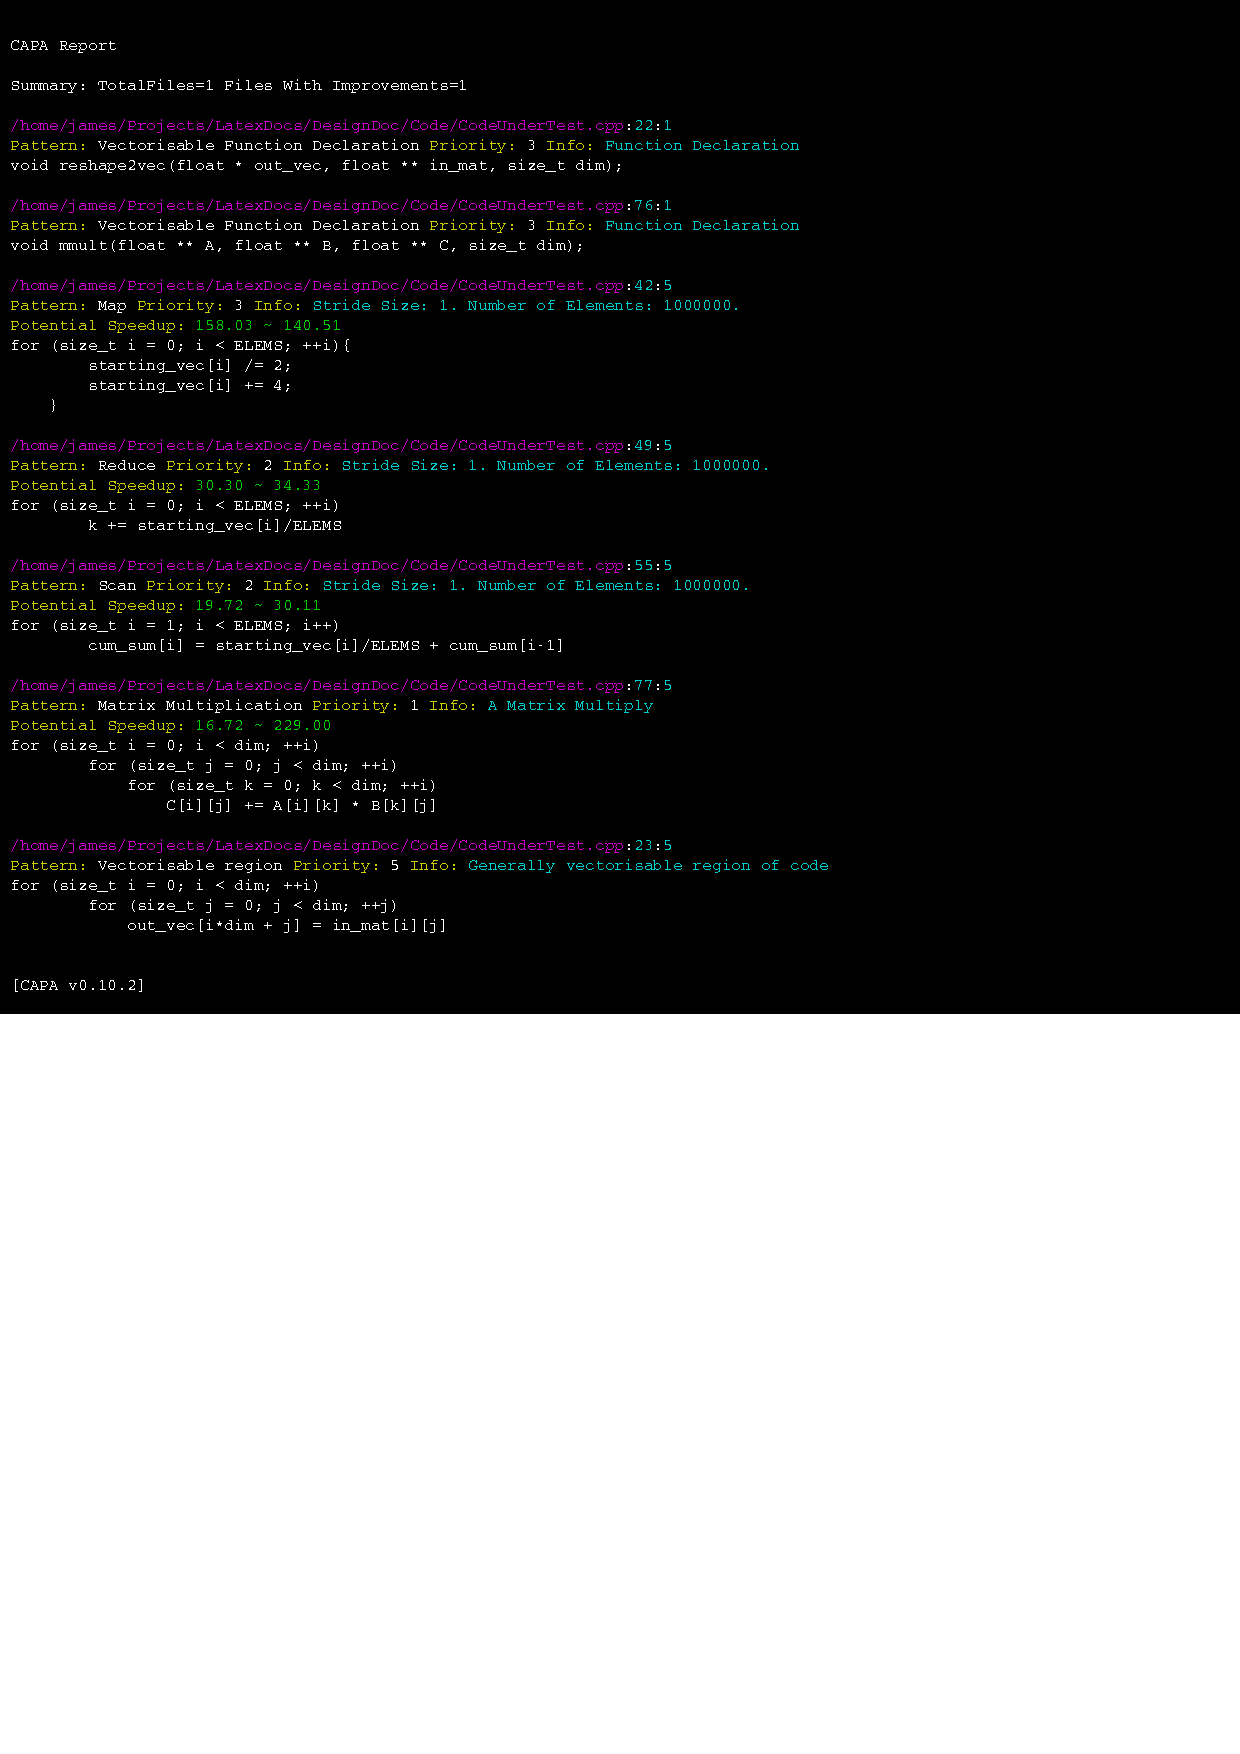
\includegraphics[clip, trim=0cm 12.7cm 6cm 0.5cm, width=\textwidth]{./Misc/report.pdf}
\caption{CAPA Generated Report}
\end{figure}
Please note that the cast study requires knowledge of the Clang AST, the output AST dump for the file
under test can be found in the Appendix at section \ref{AST}.

\subsection{Setup}
The initial setup is mostly taken care of by existing Clang and LLVM libraries. Clang Libtooling is
responsible for parsing and lexing the source file, CAPA merely passes the arguments through to the
correct Clang libraries. During the setup CAPA dynamically loads Rules for AST analysis and
Reporters for reporting. Once the rules and reporters have been loaded, CAPA loads the benchmark
information for use in the reporting phase.

Loading of rules consists of two phases. Rule Generation and Collection. Rule Generation is the
setup process whereby the AST Matchers are created, and the resulting matcher is then forwarded onto
Clang with a callback function for later processing. The rules are then collected by CAPA for
dispatching callbacks correctly.

Once the file has been loaded by the Clang front-end, parsed, and the AST constructed, the
Libtooling library begins to traverse the AST searching for a match.

\subsection{Matching}
When Clang finds a portion of the AST which matches the requirements described by the rules, the
callback function is envoked and the relevant rule must process the matching AST Node.

For our code under test, the first callback that occurs is not shown in the report, this is due to
the tag which tells CAPA to ignore that function. Further information can be found here
\ref{TaggedRegion}.

\subsubsection{Match 1: Vectorisable Function Declaration}
The first match to be reported is the result of the function declaration on line 22. The pattern
identified is a \lstinline{Vectorisable Function Declaration}. This is the simplest of all the
parallel matchers. A function declaration is deemed to be potentially vectorisable based purely on
the type information available. Vectorisable functions require an arity of at least two, with one
argument being a pointer or array type, and the other argument being a \lstinline{size_t}. This is the
most speculative of the patterns identified by CAPA, as there is very little information to work
with in a function declaration, however functions that operate on vectors in C require both a
pointer to the vector, and some information about the size of the vector, thus with that limited
information we can construct a matcher.

The matcher for this rule is described by:
\lstinputlisting[linerange={56-60}]{/home/james/Projects/CAPA/CAPA-rules/rules/parallel/VectorFunctionDeclRule.cpp}
The grammar here is quite simple, the matcher is requesting a callback if a function declaration is
found which has a parameter that is either an array type or a pointer type, and has any parameter
which is a \lstinline{size_t}. If this is found it is to be bound by the name \lstinline{Function}
and the callback will provide the bound nodes and additional AST context.

\paragraph{Match 2: Vectorisable Function Declaration}
The second match is also a \lstinline{Vectorisable Function Declaration}. This match however is a
the result of catching a function declaration on line 76. The process by which this function is
found is no different from the prior example. Note however that the types are different, and in this
case the matcher is in fact catching types with two levels of indirection. This rule is general
enough that it is capable of catching arbitrary levels of indirection.

\subsubsection{Match 3: Map Operation}
The third match to be reported is a map operation, which is identified on line 42. The reported
information for \lstinline{Map} operations is more thorough than the information provided for
\lstinline{Vectorisable Function Declaration}, this is because more information is available to the
callback due to a stronger grammar.
\lstinputlisting[linerange={155-165}]{/home/james/Projects/CAPA/CAPA-rules/rules/parallel/MapRule.cpp}
The Map matcher utilises the combinator library designed for this project in order to simplify the
top level expression. Our matcher is looking to identify loops which have an assignment where there
is a vector on both sides of the operator, or loops which have a compound binary operator and some
numeric literal. This describes most of the semantic restrictions a map operation enforces upon a
programmer however in order to extract performance information extra bindings are required.

The report states that there are 1 million elements to be processed, in order to extract this
information, the \lstinline{ForLoop} combinator provides a binding on the conditional which is
exposed in the callback. Similarly the number of elemts is also bound to by the \lstinline{ForLoop}
combinator with the respective node being exposed to the callback.

Upon a successful match, the callback function is called with the results structure. The results
structure contains all the bound nodes, as well as the AST Context. These tools are utilised in the
callback to filter out false positives, cases where the grammar of the matcher specification is not
strict enough to ensure only valid cases are matched. Within the callback the results are
re-organised into a simple class which defines a few basic operations. In order for a match to be
validated as truly representative of a Map operation, the results must be verified. This is done
through the \lstinline{MapInfo.isMap()} method, which confirms that the bound index's of the input
and ouput vectors are related without a data dependency.

Beyond validating matches, the callback is responsible for retrieving and providing information to
the reporters about the known quantities of the region. That is to say that the callback is
responsible for retrieving whatever information is available from the now exposed bound nodes.  In
order to calculate the number of elements to be processed, the right hand side of the loop condition
is constant folded to an integer. If this is possible and there is a result, that information is
then used as the number of elements to process. Similarly the stride size in the report is 1. This
is also bound by the \lstinline{ForLoop} combinator, which binds to the loop increment. This binding
is then matched against typical loop increment expressions, and where possible constant folding
extracts the stride size.

This information is then passed along to the reporter in order to provide performance metrics.

\subsubsection{Match 4: Reduce Operation}
The fourth match to be reported is a reduction, which occurs on line 49. Like the Map report, the
reduction provides more information about potential improvements. The reduction in the code under
test is the calculating of a mean, by summing the contents of the \lstinline{starting_vec} divided
by the number of elements. This is cleary a many to one operation which satisfies the requirements
of parallel reductions. 
\lstinputlisting[linerange={148-157}]{/home/james/Projects/CAPA/CAPA-rules/rules/parallel/ReduceRule.cpp}


\subsection{Tagged Regions}\label{TaggedRegion}
%------------------------------------------------



